\newacronym{tclab}{TCLab}{\textit{Temperature Control Lab}}
\newacronym{tclabsp}{TCLabSP}{\textit{Temperature Control Lab Sao Paulo}}
\newacronym{byu}{BYU}{\textit{Brigham Young University}}
\newacronym{ncsu}{NCSU}{\textit{North Carolina State University}}
\newacronym{si}{SI}{Sistema Internacional de Unidades}

\chapter{Planta piloto}
\label{ch:planta_piloto}

% =====================================================================================================
% ============================================= Section ===============================================
% =====================================================================================================
\section{TCLab}
\label{sec:tclab}

O equipamento utilizado para o projeto de ações de controle é um mini sistema chamado \acrlong{tclab}
(do inglês, Laboratório de Controle de Temperatura), ou apenas \acrshort{tclab}\footnote{                       % footnote
	Maiores informações sobre o \acrshort{tclab} podem ser encontrados em
	\href{http://apmonitor.com/heat.htm}{http://apmonitor.com/heat.htm}.
}(\cref{fig:tclab}). Esse sistema foi desenvolvido na \acrlong{byu} (\acrshort{byu}) e apresentado
pela primeira vez no \textit{2017 ASEE Summer School}, na \acrlong{ncsu} (\acrshort{ncsu}). Foi
desenvolvido com o propósito de facilitar o acesso de estudantes a um laboratório de testes de controle.

Esse equipamento é essencialmente um \textit{shield} para Arduino\footnote{
    Arduino é uma plataforma de prototipagem eletrônica de hardware livre e de placa única, projetada com um    % footnote
    microcontrolador Atmel AVR com suporte de entrada/saída embutido.                                           % footnote
} contendo 2 aquecedores e 2 sensores de temperatura, indicados na \cref{fig:tclab_description}. A energia dos aquecedores é
transferida através de condução, convecção e radiação até os sensores de temperatura. Tanto o controle da
potência dos aquecedores quanto as medições realizadas pelos sensores são efetuados através do Arduino.

O \acrshort{tclab} permite que a programação de controle do sistema possa ser feito utilizando linguagem Python,
\acrshort{matlab} ou Simulink.

\begin{figure}[h]
	\caption{Laboratório de Controle de Temperatura}
	\begin{center}
		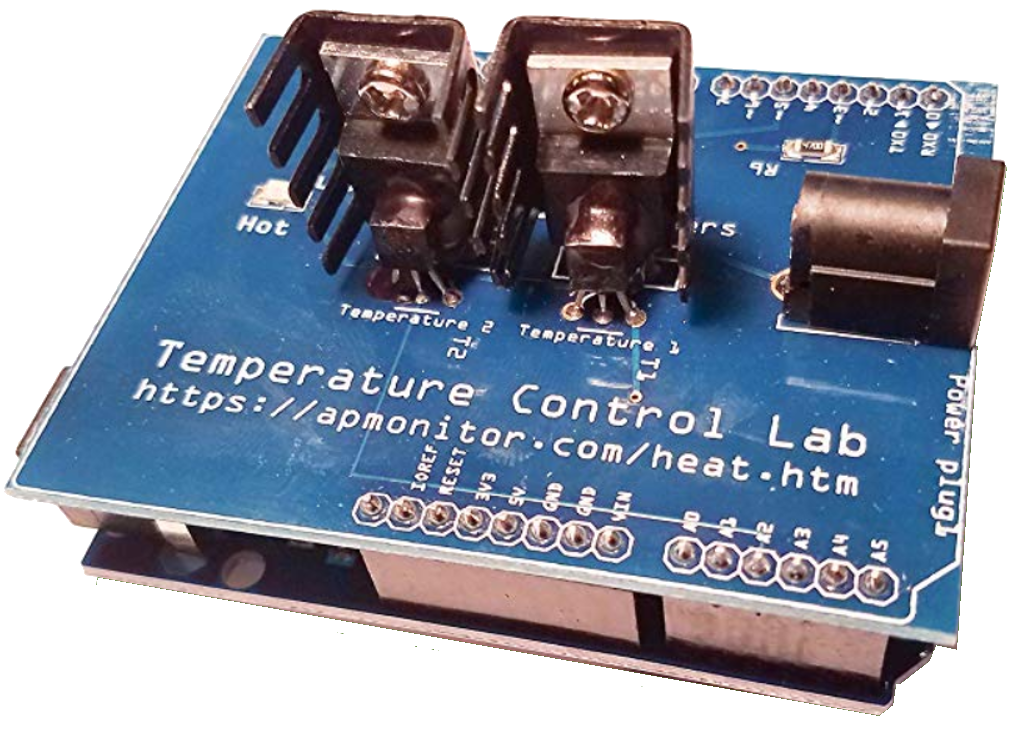
\includegraphics[width=0.45\textwidth]{./5_images/tclab.png} 
		\label{fig:tclab}
	\end{center}
	\centering
	\makebox[\width]{Fonte: \citeonline{Hedengrena}} 
\end{figure}

\begin{figure}[h]
	\caption{Componentes principais do TCLab}
	\begin{center}
		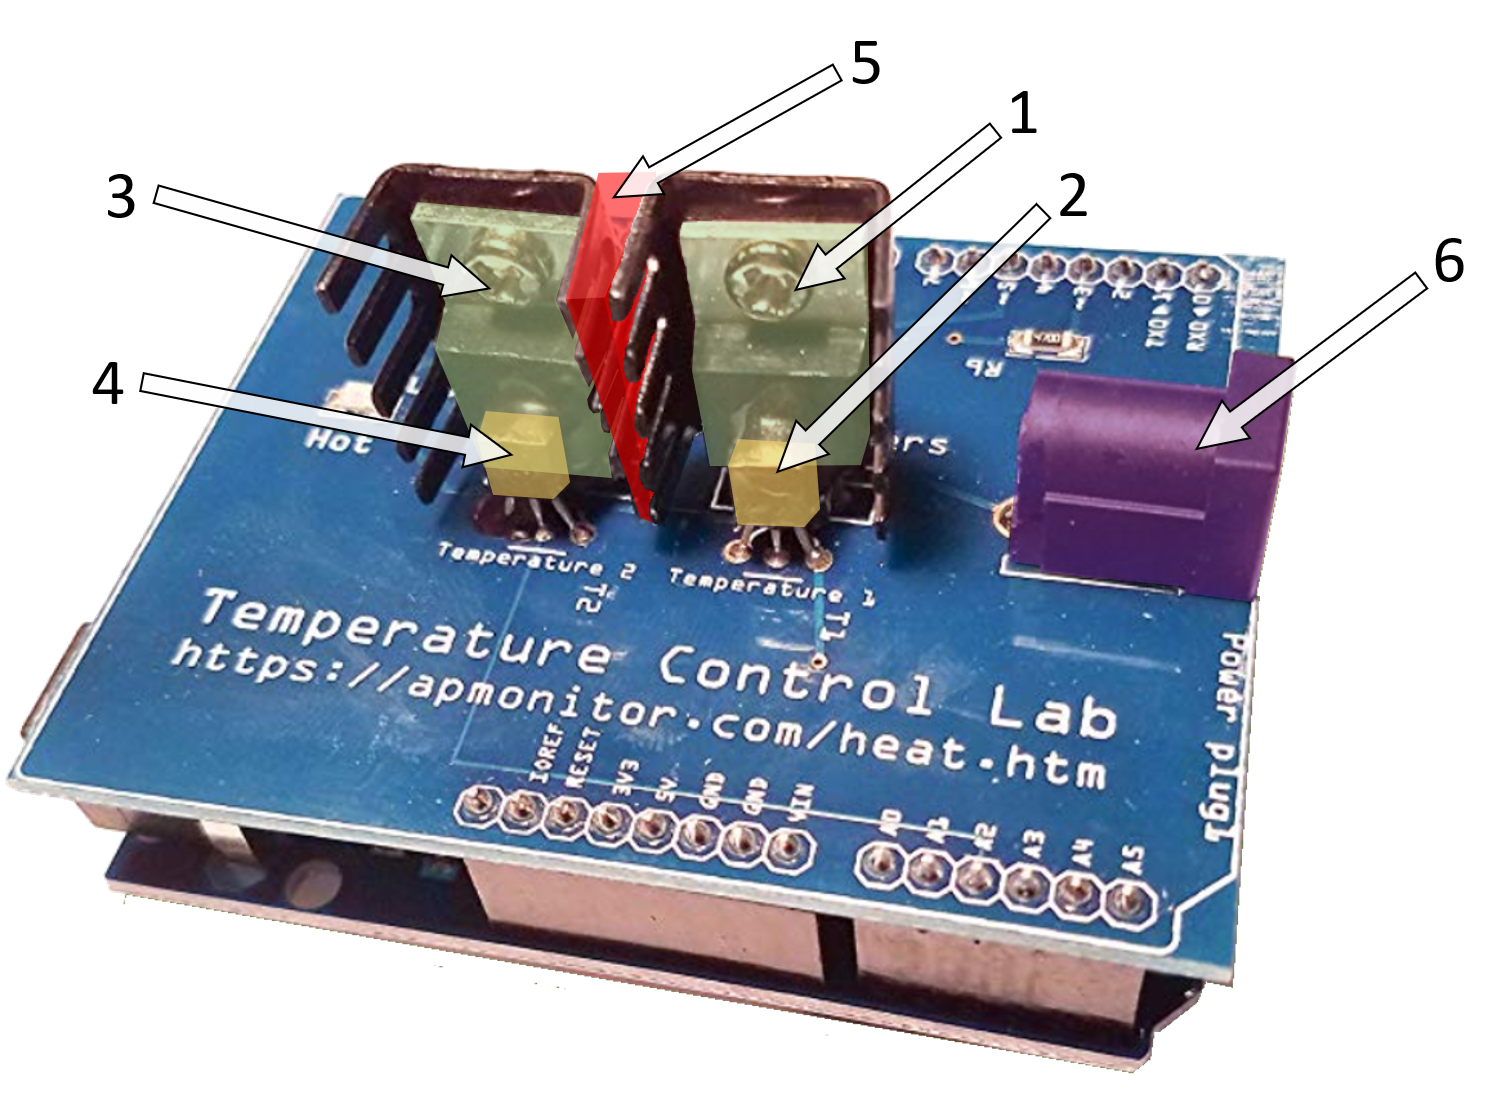
\includegraphics[width=0.45\textwidth]{./5_images/tclab_color_numbers.png} 
		\label{fig:tclab_description}
	\end{center}
	\centering
	\makebox[\width]{Fonte: \citeonline{Prata2019}, adaptado de \citeonline{Hedengrena}} 
\end{figure}

\begin{table}[h]
	\centering
	\caption{Componentes principais do TCLab}
	\label{tab:componentes_tclabsp}
	\begin{tabular}{cl} \toprule
		{Item}			& {Descrição} 									\\ \midrule
		1		 		& Aquecedor 1 ($T_{H1}$)		 				\\
		2				& Sensor de temperatura 1 ($T_{C1}$)			\\
		3				& Aquecedor 2 ($T_{H2}$)						\\
		4				& Sensor de temperatura 2 ($T_{C2}$)			\\
		5				& Superfície entre dissipadores [2 $cm^2$]		\\
		6				& Entrada para alimentação						\\ \bottomrule
	\end{tabular}
	\caption*{Fonte: \citeonline{Prata2019}}
\end{table}

% =====================================================================================================
% ============================================= Section ===============================================
% =====================================================================================================
\section{Planta piloto - TCLabSP}
\label{sec:planta_piloto}

A planta piloto desenvolvida para esse projeto é chamada de \acrlong{tclabsp}, ou apenas \acrshort{tclabsp},
e consiste em um envólucro em acrílico que foi construído com o intuito de minimizar interferências
externas e de possibilitar um maior controle dos distúrbios, uma vez que ventiladores foram incluídos
ao sistema, juntamente com o \acrshort{tclab} apresentado na \cref{sec:tclab}.

\begin{figure}[h]
    \centering
	\caption{Visão geral da Planta Piloto - TCLabSP}
    \begin{minipage}{0.47\textwidth}
        \centering
        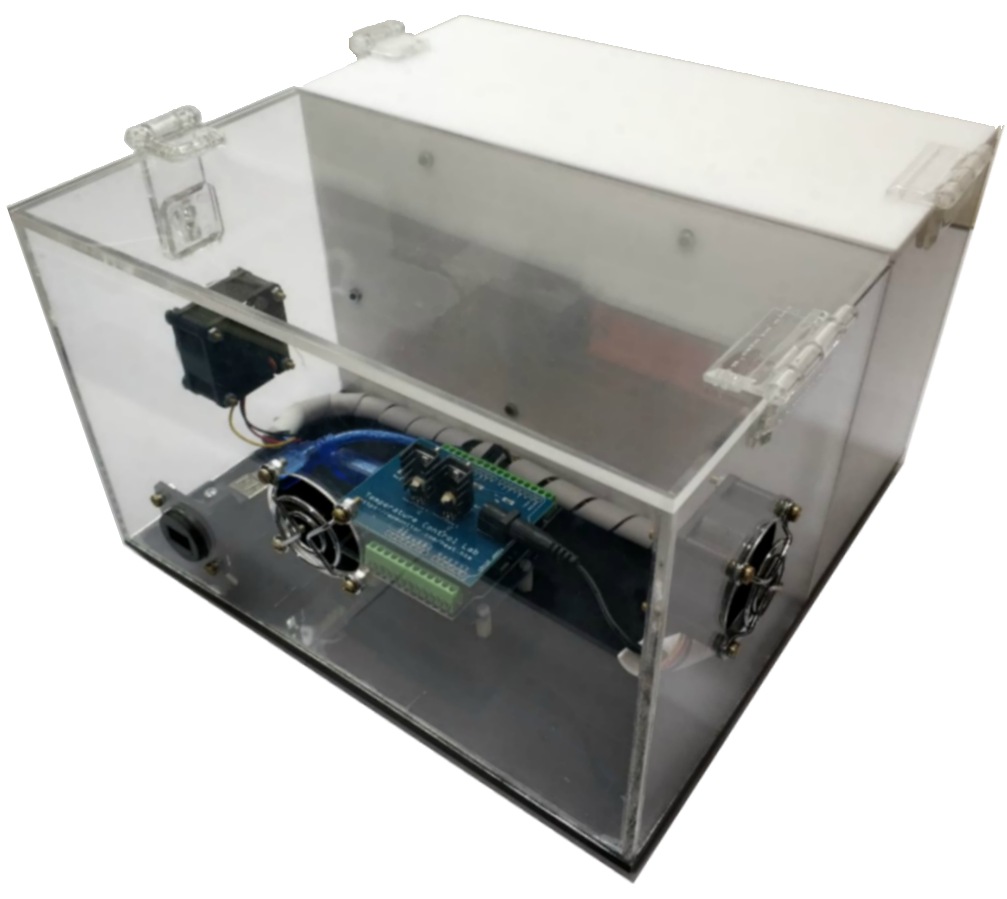
\includegraphics[width=0.9\textwidth]{./5_images/TCLabSP_1.png} 
    \end{minipage}\hfill
    \begin{minipage}{0.47\textwidth}
        \centering
        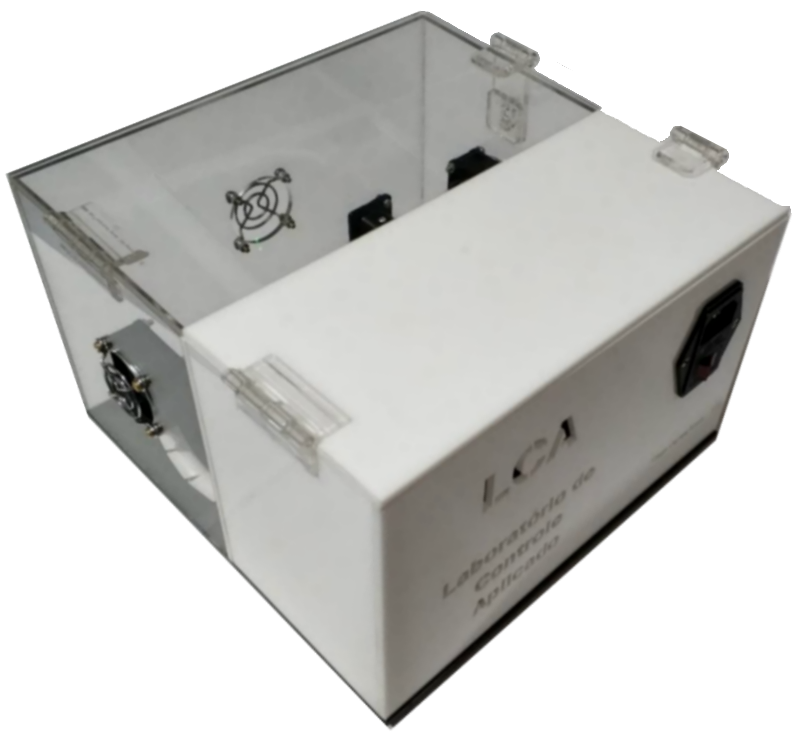
\includegraphics[width=0.9\textwidth]{./5_images/TCLabSP_2.png} 
	\end{minipage}
	\label{fig:tclabsp}		      
	Fonte: \citeonline{Prata2019}
\end{figure}

A \cref{fig:tclabsp} apresenta uma visão geral da \acrshort{tclabsp}, enquanto a \cref{fig:tclabsp_color}
e a \cref{tab:componentes_tclabsp} detalham seus componentes principais.

\begin{figure}[h]
	\caption{Componentes principais do TCLabSP}
	\begin{center}
		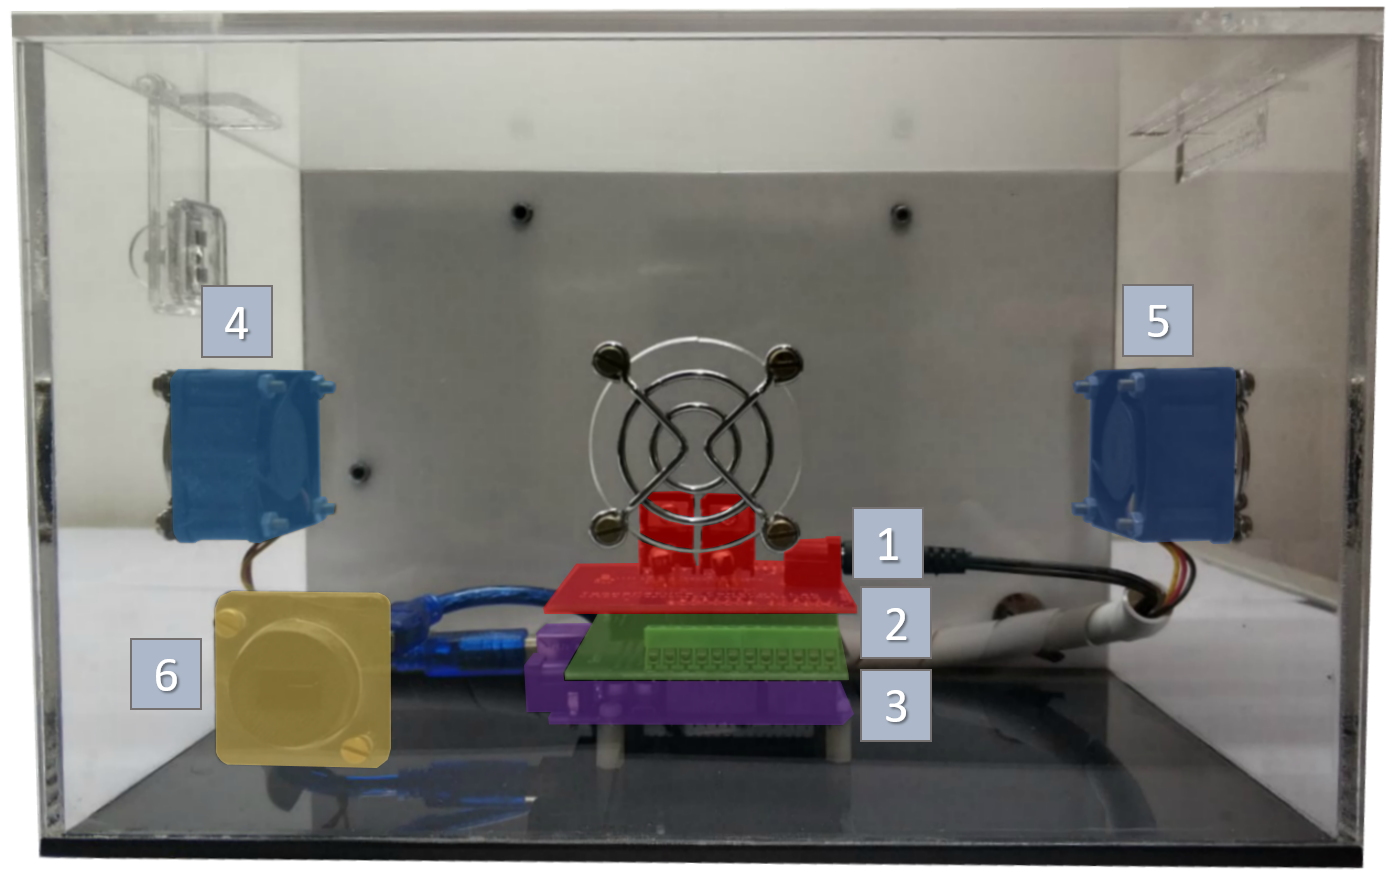
\includegraphics[width=0.65\textwidth]{./5_images/TCLabSP_color_numbers.png} 
		\label{fig:tclabsp_color}
	\end{center}
	\centering
	\makebox[\width]{Fonte: \citeonline{Prata2019}} 
\end{figure}

\begin{table}[!h]
	\centering
	\caption{Componentes principais do TCLabSP}
	\label{tab:componentes_tclabsp}
	\begin{tabular}{cl} \toprule
		{Item}			& {Descrição} 										\\ \midrule
		1		 		& \acrshort{tclab}	 								\\
		2				& \textit{Shield} para ligação dos ventiladores		\\
		3				& Arduino Uno										\\
		4				& Ventilador 1										\\
		5				& Ventilador 2										\\
		6				& Conector mini USB									\\ \bottomrule
	\end{tabular}
	\caption*{Fonte: \citeonline{Prata2019}}
\end{table}

% =====================================================================================================
% ============================================= Section ===============================================
% =====================================================================================================
\section{Modelagem teórica da planta piloto}
\label{sec:modelagem_da_planta_piloto}

O balanço energético da \acrshort{tclab} pode ser obtido em sua documentação e
a \cref{eq:tclab_modelo_mimo} apresenta os modelos
para um sistema \acrshort{mimo}, onde ambos os aquecedores e sensores são utilizados,
sendo que, para isso, deve-se assumir que: os aquecedores e o sensores de temperatura estão na
mesma temperatura; que o efeito da condução de calor é desprezado e que as únicas trocas de
calor acontecem através de radiação ou convecção; que o aquecedor inicialmente está desligado
e que tanto o aquecedor quanto o sensor inicialmente estão em temperatura ambiente.

\begin{subequations}
	\label{eq:tclab_modelo_mimo}
	\begin{gather}
		mC_p \dfrac{dT_{H1}}{dt} = UA (T_{\infty} - T_{H1}) + \epsilon \sigma A (T_{\infty}^{4} - T_{H1}^{4}) + Qc_{12} + Qr_{12} + \alpha_1 Q_1		\label{eq:tclab_modelo_mimo_a} \\
		mC_p \dfrac{dT_{H2}}{dt} = UA (T_{\infty} - T_{H2}) + \epsilon \sigma A (T_{\infty}^{4} - T_{H2}^{4}) + Qc_{21} + Qr_{21} + \alpha_2 Q_2		\label{eq:tclab_modelo_mimo_b} \\
		\tau \dfrac{dT_{C1}}{dt} = T_{H1} - T_{C1}								\\
		\tau \dfrac{dT_{C2}}{dt} = T_{H2} - T_{C2}								\\
		Qc_{12} = U_s A_s (T_{H2} - T_{H1})							\nonumber	\\
		Qc_{21} = U_s A_s (T_{H1} - T_{H2})							\nonumber	\\
		Qr_{12} = \epsilon \sigma A_s (T_{H2}^{4} - T_{H1}^{4})		\nonumber	\\
		Qr_{21} = \epsilon \sigma A_s (T_{H1}^{4} - T_{H2}^{4})		\nonumber
	\end{gather}
\end{subequations}

A \cref{tab:tclab_modelo_mimo_valores} indica a descrição de cada uma das siglas da
\cref{eq:tclab_modelo_mimo} e também apresenta o valor de cada um.

\begin{table}[h]
	\centering
	\caption{Valores para modelagem \acrshort{mimo} do \acrshort{tclab}}
	\label{tab:tclab_modelo_mimo_valores}
	\begin{tabular}{cccc} \toprule
		{Sigla} 		& {Descrição} 							& {Valor} 											& {Valor (\acrshort{si})} 							\\ \midrule
		$T_{H1}$ 		& Temperatura do aquecedor 1			& - 												& -													\\
		$T_{C1}$ 		& Temperatura do sensor 1				& - 												& -													\\
		$T_{H2}$ 		& Temperatura do aquecedor 2			& - 												& -													\\
		$T_{C2}$ 		& Temperatura do sensor 2				& - 												& -													\\
		$T_{0}$ 		& Temperatura inicial 					& $20^\circ C$ 										& $293{,}15 K $										\\
		$T_{\infty}$	& Temperatura ambiente					& $20^\circ C$										& $293{,}15 K $										\\
		$Q_1$			& Saída do aquecedor 1					& $0$ à $100\%$										& $0$ à $100\%$										\\
		$\alpha_1$		& Fator do aquecedor 1					& $0{,}0123$ $\sfrac{W}{\% aquec.}$				& $0{,}0123$ $\sfrac{W}{\% aquec.}$						\\
		$Q_2$			& Saída do aquecedor 2					& $0$ à $100\%$										& $0$ à $100\%$										\\
		$\alpha_2$		& Fator do aquecedor 2					& $0{,}0062$ $\sfrac{W}{\% aquec.}$				& $0{,}0062$ $\sfrac{W}{\% aquec.}$						\\
		$C_p$			& Capacidade de aquecimento				& $500$ $\sfrac{J}{kg.K}$							& $500$ $\sfrac{J}{kg.K}$							\\
		$A$				& Área de superfície					& $10 cm^{2}$										& $1{\times}10^{-3} m^{2}$							\\
		$A_s$			& Idem $A$ porém entre aquecedores		& $2 cm^{2}$										& $2{\times}10^{-4} m^{2}$							\\
		$m$				& Massa									& $4 g$												& $0{,}004 kg	$									\\
		$\tau$			& Constante de tempo de condução		& $20{,}3 s$										& $20{,}3 s$										\\
		$U$				& Coef. global de transf. de calor		& $4{,}7$ $\sfrac{W}{m^{2}K}$						& $4{,}7$ $\sfrac{W}{m^{2}K}$						\\
		$U_s$			& Idem $U_s$ porém entre aquecedores	& $15{,}45$ $\sfrac{W}{m^{2}K}$						& $15{,}45$ $\sfrac{W}{m^{2}K}$						\\
		$\epsilon$		& Emissividade							& $0{,}9$											& $0{,}9$											\\
		$\sigma$		& Constante de Stefan Boltzmann			& $5{,}67{\times}10^{-8}$ $\sfrac{W}{m^{2}K^{4}}$	& $5{,}67{\times}10^{-8}$ $\sfrac{W}{m^{2}K^{4}}$	\\ \bottomrule
	\end{tabular}
	\caption*{Fonte: Autor, adaptado de \citeonline{Hedengrena}}
\end{table}

A partir da \cref{eq:tclab_modelo_mimo} é possível elaborar o modelo de espaço de estados teórico.
Para isso assume-se que os estados são $T_{H1}$, $T_{H2}$, $T_{C1}$ e $T_{C2}$, todos linearizados
por expansões em séries de Taylor.

O modelo de espaço de estados teórico tem a forma:

\begin{equation*}
	\begin{aligned}
		\dot{x} &= Ax + Bu		\\
		y &= Cx + Du
	\end{aligned}
\end{equation*}	

\noindent
Sendo:

\begin{equation}
	\begin{aligned}
		\begin{bmatrix}
			\dot{T}_{H1}^{'}	\\
			\dot{T}_{H2}^{'}	\\
			\dot{T}_{C1}^{'}	\\
			\dot{T}_{C2}^{'}
		\end{bmatrix}
		&=&
		\begin{bmatrix}
			a_{1,1}		&		a_{1,2}		&		a_{1,3}		&		a_{1,4}		\\
			a_{2,1}		&		a_{2,2}		&		a_{2,3}		&		a_{2,4}		\\
			a_{3,1}		&		a_{3,2}		&		a_{3,3}		&		a_{3,4}		\\
			a_{4,1}		&		a_{4,2}		&		a_{4,3}		&		a_{4,4}	
		\end{bmatrix}
		&
		\begin{bmatrix}
			T_{H1}^{'}	\\
			T_{H2}^{'}	\\
			T_{C1}^{'}	\\
			T_{C2}^{'}
		\end{bmatrix}
		+&
		\begin{bmatrix}
			b_{1,1}		&		b_{1,2}		\\
			b_{2,1}		&		b_{2,2}		\\
			b_{3,1}		&		b_{3,2}		\\
			b_{4,1}		&		b_{4,2}	
		\end{bmatrix}
		&
		\begin{bmatrix}
			Q_{1}^{'}		\\
			Q_{2}^{'}
		\end{bmatrix}
		\\
		\\
		\begin{bmatrix}
			T_{C1}^{'}	\\
			T_{C2}^{'}
		\end{bmatrix}
		&=&
		\begin{bmatrix}
			0	&	0	&	1	&	0	\\
			0	&	0	&	0	&	1
		\end{bmatrix}
		&
		\begin{bmatrix}
			T_{H1}^{'}	\\
			T_{H2}^{'}	\\
			T_{C1}^{'}	\\
			T_{C2}^{'}
		\end{bmatrix}
		+&
		\begin{bmatrix}
			0	&	0	\\
			0	&	0
		\end{bmatrix}
		&
		\begin{bmatrix}
			Q_{1}^{'}		\\
			Q_{2}^{'}
		\end{bmatrix}
	\end{aligned}
\end{equation}

\noindent
Onde:
\begin{equation*}
	\begin{aligned}
		a_{1,1} &= \left. \frac{\partial f_1}{\partial T_{H1}} \right|_{\overline{Q},\overline{T}} = 
				  - \frac{UA + 4 \epsilon \sigma A T_0^3 + U_s A_s + 4 \epsilon \sigma A_s T_0^3}{m C_p} = 
				  -0.00698		
				  \\
		a_{1,2} &= \left. \frac{\partial f_1}{\partial T_{H2}} \right|_{\overline{Q},\overline{T}} = 
				  \frac{U_s A_s + 4 \epsilon \sigma A_s T_0^3}{m C_p} = 
				  0.00205
				  \\
		a_{1,3} &= \left. \frac{\partial f_1}{\partial T_{C1}} \right|_{\overline{Q},\overline{T}} = 
				  0
				  \\
		a_{1,4} &= \left. \frac{\partial f_1}{\partial T_{C2}} \right|_{\overline{Q},\overline{T}} = 
				  0
	\end{aligned}
\end{equation*}

\begin{equation*}
	\begin{aligned}
		a_{2,1} &= \left. \frac{\partial f_2}{\partial T_{H1}} \right|_{\overline{Q},\overline{T}} = 
				  \frac{U_s A_s + 4 \epsilon \sigma A_s T_0^3}{m C_p} = 
				  0.00205
				  \\
		a_{2,2} &= \left. \frac{\partial f_2}{\partial T_{H2}} \right|_{\overline{Q},\overline{T}} = 
				  - \frac{UA + 4 \epsilon \sigma A T_0^3 + U_s A_s + 4 \epsilon \sigma A_s T_0^3}{m C_p} = 
				  -0.00698		
				  \\
		a_{2,3} &= \left. \frac{\partial f_2}{\partial T_{C1}} \right|_{\overline{Q},\overline{T}} = 
				  0
				  \\
		a_{2,4} &= \left. \frac{\partial f_2}{\partial T_{C2}} \right|_{\overline{Q},\overline{T}} = 
				  0
	\end{aligned}
\end{equation*}

\begin{equation*}
	\begin{aligned}
		a_{3,1} &= \left. \frac{\partial f_3}{\partial T_{H1}} \right|_{\overline{Q},\overline{T}} = 
				  \frac{1}{\tau} =
				  0.04926
				  \\
		a_{3,2} &= \left. \frac{\partial f_3}{\partial T_{H2}} \right|_{\overline{Q},\overline{T}} = 
				  0
				  \\
		a_{3,3} &= \left. \frac{\partial f_3}{\partial T_{C1}} \right|_{\overline{Q},\overline{T}} = 
				  - \frac{1}{\tau} =
				  - 0.04926
				  \\
		a_{3,4} &= \left. \frac{\partial f_3}{\partial T_{C2}} \right|_{\overline{Q},\overline{T}} = 
				  0
	\end{aligned}
\end{equation*}

\begin{equation*}
	\begin{aligned}
		a_{4,1} &= \left. \frac{\partial f_4}{\partial T_{H1}} \right|_{\overline{Q},\overline{T}} = 
				  0
				  \\
		a_{4,2} &= \left. \frac{\partial f_4}{\partial T_{H2}} \right|_{\overline{Q},\overline{T}} = 
				  \frac{1}{\tau} =
				  0.04926
				  \\	
		a_{4,3} &= \left. \frac{\partial f_4}{\partial T_{C1}} \right|_{\overline{Q},\overline{T}} = 
				  0
				  \\
		a_{4,4} &= \left. \frac{\partial f_4}{\partial T_{C2}} \right|_{\overline{Q},\overline{T}} = 
				  - \frac{1}{\tau} =
				  - 0.04926
	\end{aligned}
\end{equation*}

\begin{equation*}
	\begin{aligned}
		b_{1,1} &= \left. \frac{\partial f_1}{\partial T_{Q1}} \right|_{\overline{Q},\overline{T}} = 
				  \frac{\alpha_1}{m C_p} =
				  0.00615
				  \\
		b_{1,2} &= \left. \frac{\partial f_1}{\partial T_{Q2}} \right|_{\overline{Q},\overline{T}} = 
				  0
	\end{aligned}
\end{equation*}

\begin{equation*}
	\begin{aligned}
		b_{2,1} &= \left. \frac{\partial f_2}{\partial T_{Q1}} \right|_{\overline{Q},\overline{T}} = 
				  0
				  \\
		b_{2,2} &= \left. \frac{\partial f_2}{\partial T_{Q2}} \right|_{\overline{Q},\overline{T}} = 
				  \frac{\alpha_2}{m C_p} =
				  0.00310
	\end{aligned}
\end{equation*}

\begin{equation*}
	\begin{aligned}
		b_{3,1} &= \left. \frac{\partial f_3}{\partial T_{Q1}} \right|_{\overline{Q},\overline{T}} = 
				  0
				  \\
		b_{3,2} &= \left. \frac{\partial f_3}{\partial T_{Q2}} \right|_{\overline{Q},\overline{T}} = 
				  0
	\end{aligned}
\end{equation*}

\begin{equation*}
	\begin{aligned}
		b_{4,1} &= \left. \frac{\partial f_4}{\partial T_{Q1}} \right|_{\overline{Q},\overline{T}} = 
				  0
				  \\
		b_{4,2} &= \left. \frac{\partial f_4}{\partial T_{Q2}} \right|_{\overline{Q},\overline{T}} = 
				  0
	\end{aligned}
\end{equation*}

\noindent
Assim temos:

\begin{equation}
	\label{eq:tclab_modelo_teorico}
	\begin{aligned}
		\begin{bmatrix}
			\dot{T}_{H1}^{'}	\\
			\dot{T}_{H2}^{'}	\\
			\dot{T}_{C1}^{'}	\\
			\dot{T}_{C2}^{'}
		\end{bmatrix}
		&=&
		\begin{bmatrix}
			-0.00698		&		0.00205		&		0			&		0		\\
			0.00205			&		-0.00698	&		0			&		0		\\
			0.04926			&		0			&		-0.04926	&		0		\\
				 0			&		0.04926		&		0			&		-0.04926	
		\end{bmatrix}
		&
		\begin{bmatrix}
			T_{H1}^{'}	\\
			T_{H2}^{'}	\\
			T_{C1}^{'}	\\
			T_{C2}^{'}
		\end{bmatrix}
		+&
		\begin{bmatrix}
			0.00615		&		0		\\
			0			&		0.00310	\\
			0			&		0		\\
			0			&		0	
		\end{bmatrix}
		&
		\begin{bmatrix}
			Q_{1}^{'}		\\
			Q_{2}^{'}
		\end{bmatrix}
		\\
		\\
		\begin{bmatrix}
			T_{C1}^{'}	\\
			T_{C2}^{'}
		\end{bmatrix}
		&=&
		\begin{bmatrix}
			0	&	0	&	1	&	0	\\
			0	&	0	&	0	&	1
		\end{bmatrix}
		&
		\begin{bmatrix}
			T_{H1}^{'}	\\
			T_{H2}^{'}	\\
			T_{C1}^{'}	\\
			T_{C2}^{'}
		\end{bmatrix}
		+&
		\begin{bmatrix}
			0	&	0	\\
			0	&	0
		\end{bmatrix}
		&
		\begin{bmatrix}
			Q_{1}^{'}		\\
			Q_{2}^{'}
		\end{bmatrix}
	\end{aligned}
\end{equation}


% .....................................................................................................
% ............................................ Subsection .............................................
% .....................................................................................................
\subsection{Verificação do modelo teórico}
\label{subsec:verificacao_do_modelo_teorico}

Para a verificação do modelo teórico obtido na \cref{eq:tclab_modelo_teorico} criou-se o ambiente de
teste indicado na \cref{fig:ModeloTeorico_e_TCLabSP_Simulink} onde tanto o sistema real quanto o modelo
teórico eram excitados pelo mesmo sinal de entrada.

As motivações e o detalhamento dos sinais de excitação utilizados neste experimento são melhores abordados
posteriormente na \cref{subsec:sinais_de_excitacao} - \nameref{subsec:sinais_de_excitacao}.

\begin{figure}[h]
	\caption{Diagrama do ambiente de testes do modelo teórico}
	\begin{center}
		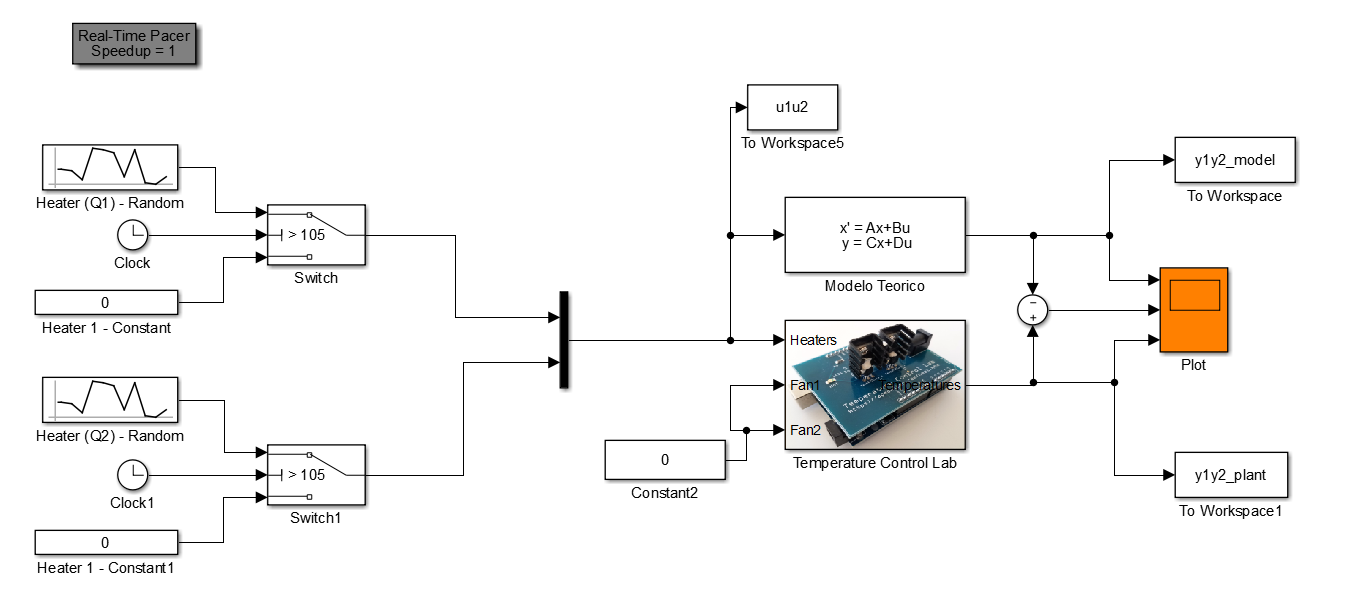
\includegraphics[width=0.95\textwidth]{./5_images/ModeloTeorico_e_TCLabSP_Simulink.png} 
		\label{fig:ModeloTeorico_e_TCLabSP_Simulink}
	\end{center}
	\centering
	\makebox[\width]{Fonte: Autor} 
\end{figure}

A comparação entre as respostas do sistema real e do modelo teórico, quando excitados em malha aberta pelos mesmos sinais
de entrada, pode ser verificada nas \cref{fig:ModeloTeorico_e_TCLabSP_y1} e \cref{fig:ModeloTeorico_e_TCLabSP_y2},
respectivamente.

Para expressar numericamente quanto este modelo obtido se aproximou da planta real durante os experimentos,
será utilizada a \cref{eq:nrmse} que também será apresentada com mais detalhes no \cref{ch:modelagem_experimental}.
A \cref{tab:ModeloTeorico_e_TCLabSP_results} apresenta esses valores.

\begin{table}[h]
	\centering
	\caption{Resultado numérico da comparação entre o modelo teórico e a planta real}
	\label{tab:ModeloTeorico_e_TCLabSP_results}
	\begin{tabular}{ll} \toprule
		{Saída}								& {fit}					\\ \midrule
		Sensor de temperatura 1				& $87.05\%$				\\
		Sensor de temperatura 2				& $67.32\%$				\\ \bottomrule
	\end{tabular}
	\caption*{Fonte: Autor}
\end{table}

\begin{figure}[h]
	\caption{Respostas real e modelada do Sensor de Temperatura 1}
	\begin{center}
		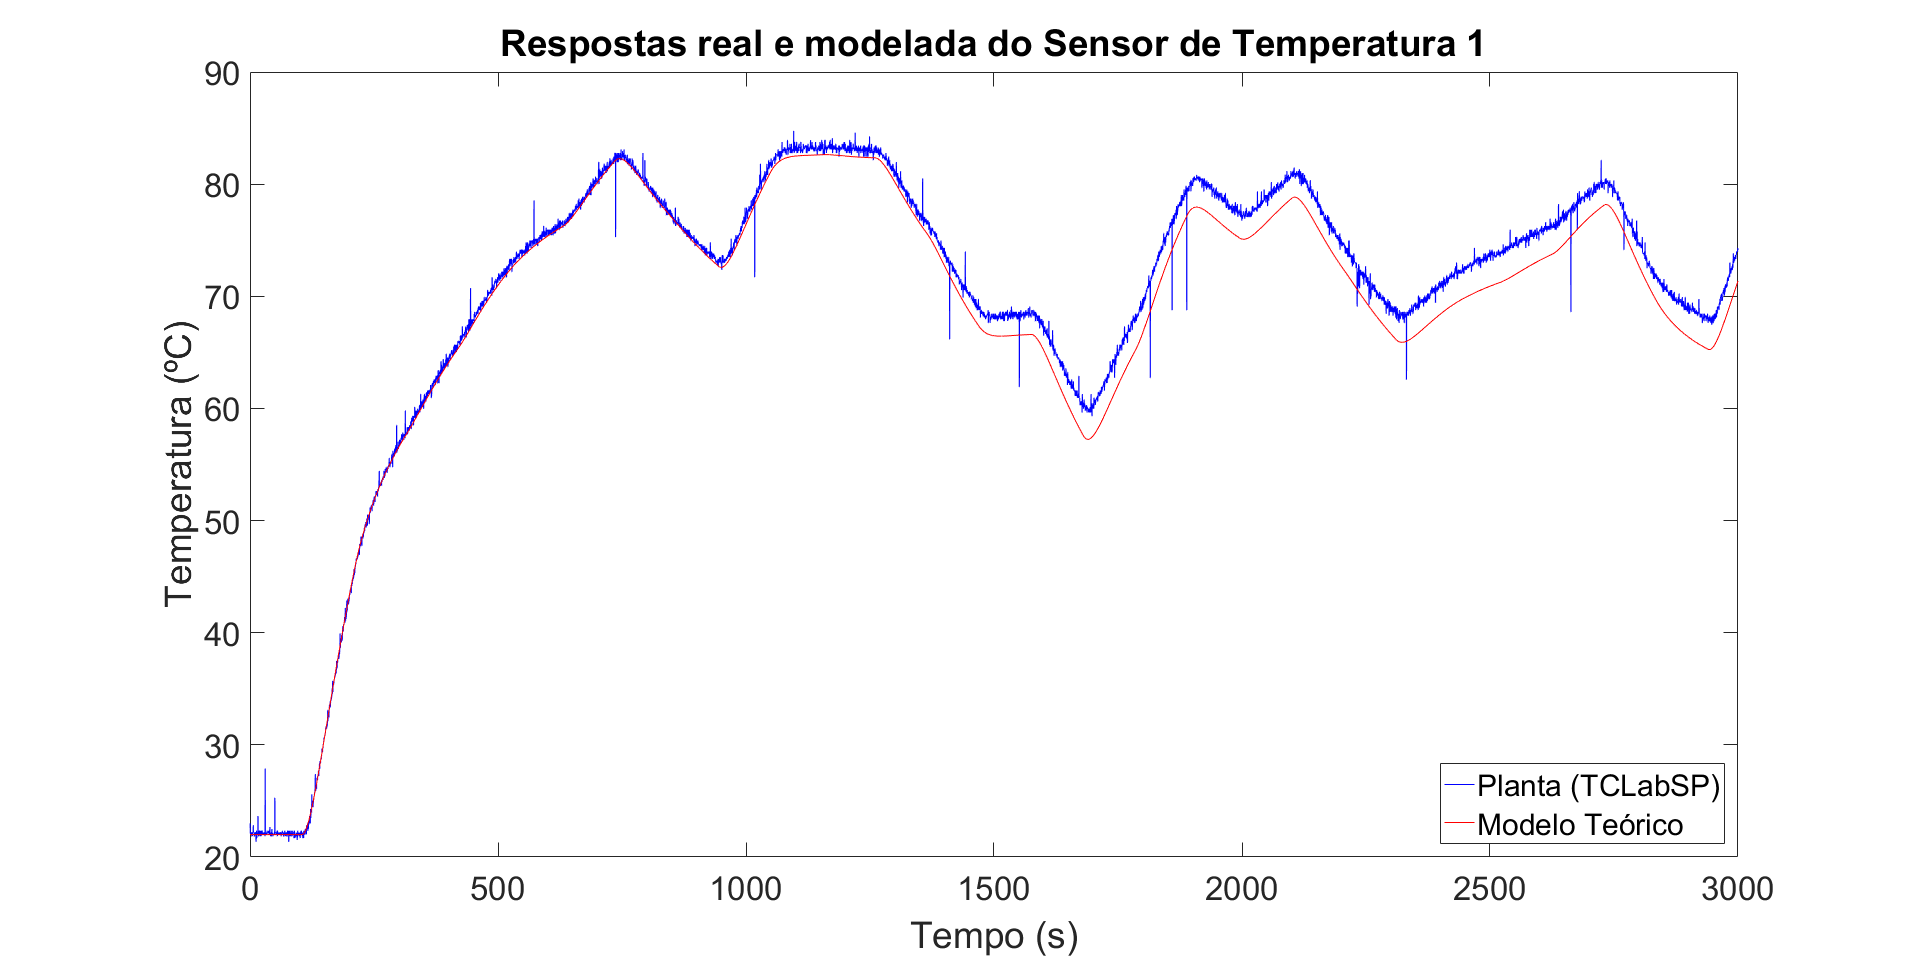
\includegraphics[width=0.95\textwidth]{./5_images/ModeloTeorico_e_TCLabSP_y1.png} 
		\label{fig:ModeloTeorico_e_TCLabSP_y1}
	\end{center}
	\centering
	\makebox[\width]{Fonte: \citeonline{Prata2019}} 
\end{figure}

\begin{figure}[h]
	\caption{Respostas real e modelada do Sensor de Temperatura 2}
	\begin{center}
		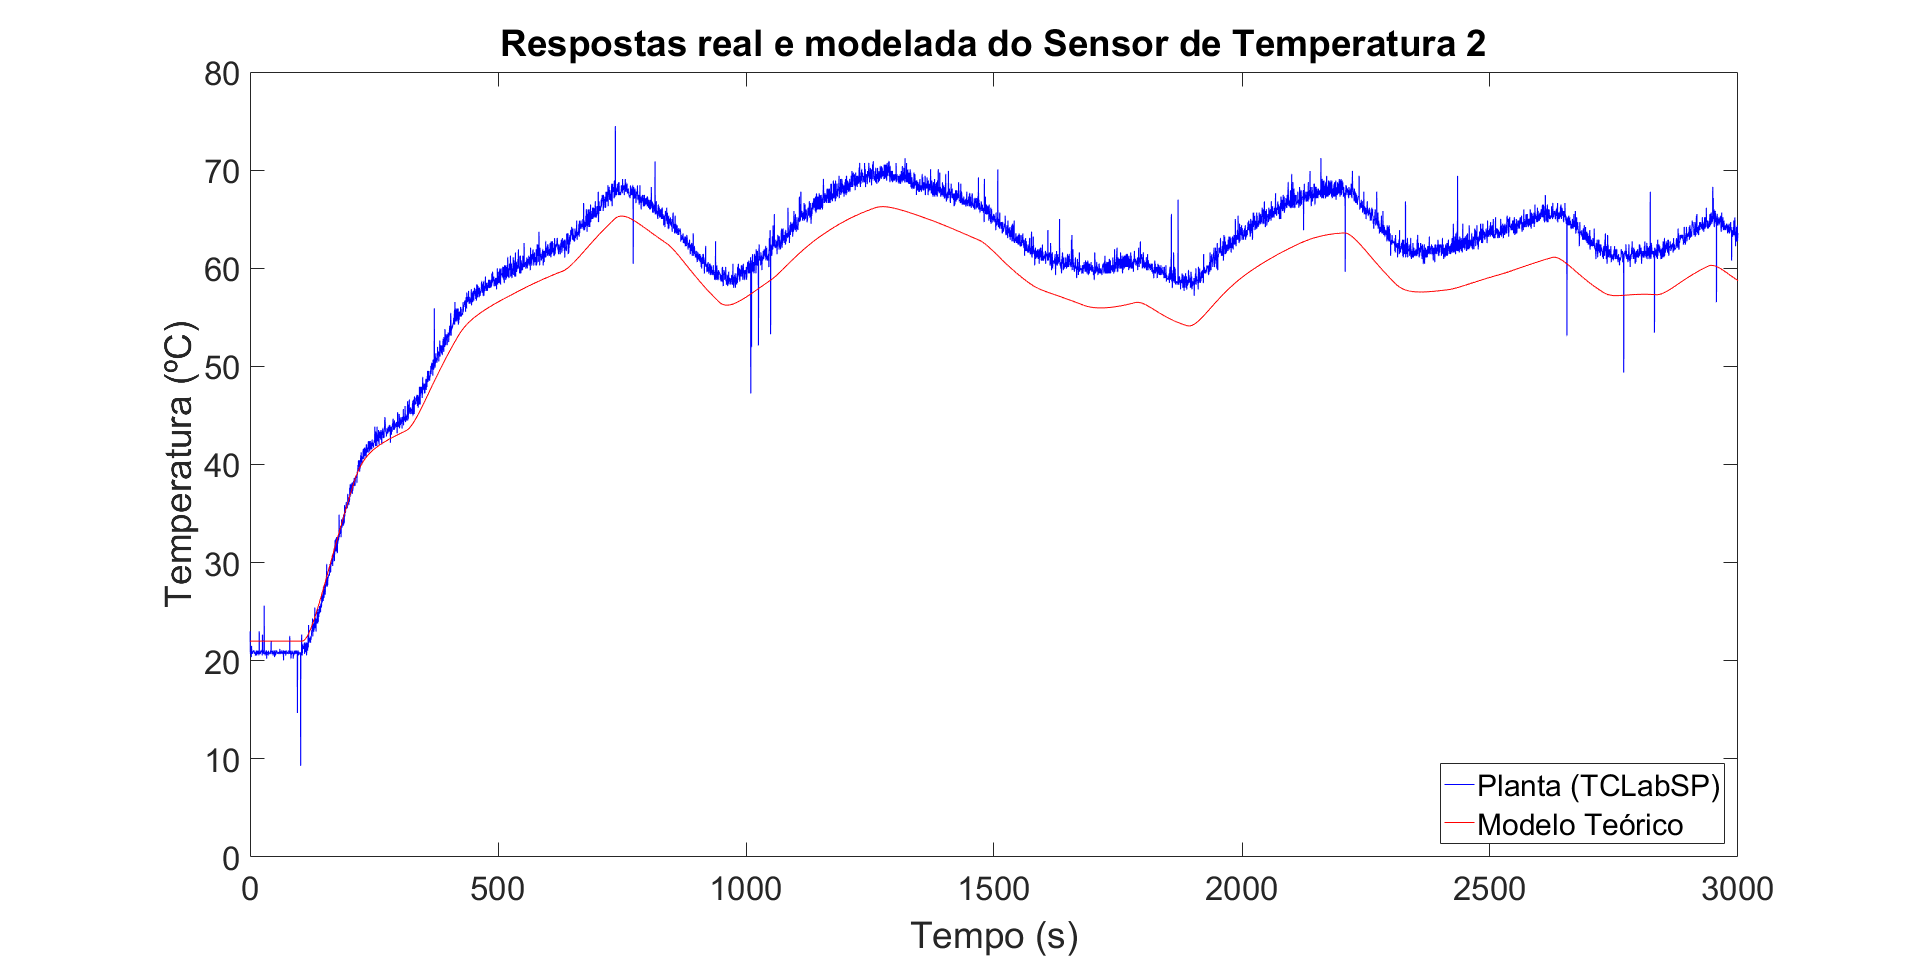
\includegraphics[width=0.95\textwidth]{./5_images/ModeloTeorico_e_TCLabSP_y2.png} 
		\label{fig:ModeloTeorico_e_TCLabSP_y2}
	\end{center}
	\centering
	\makebox[\width]{Fonte: \citeonline{Prata2019}} 
\end{figure}